% arara: indent: {overwrite: yes}
\documentclass{article}

% if you need to pass options to natbib, use, e.g.:
% \PassOptionsToPackage{numbers, compress}{natbib}
% before loading nips_2016
%
% to avoid loading the natbib package, add option nonatbib:
% \usepackage[nonatbib]{nips_2016}

\usepackage[final]{nips_2016}

% to compile a camera-ready version, add the [final] option, e.g.:
% \usepackage[final]{nips_2016}

\usepackage[utf8]{inputenc} % allow utf-8 input
\usepackage[T1]{fontenc}    % use 8-bit T1 fonts
\usepackage{hyperref}       % hyperlinks
\usepackage{url}            % simple URL typesetting
\usepackage{booktabs}       % professional-quality tables
\usepackage{amsfonts}       % blackboard math symbols
\usepackage{nicefrac}       % compact symbols for 1/2, etc.
\usepackage{microtype}      % microtypography
\usepackage{physics}		 % Physics package for derivatives
\usepackage{graphicx,float,caption,subcaption,tikz}
\usepackage[nomarkers,figuresonly]{endfloat}
\usepackage{listings}
\usepackage{color} %red, green, blue, yellow, cyan, magenta, black, white
\usepackage{animate}
\usepackage{multirow}
\usepackage{pgffor}
\usepackage{tabularx}

\usepackage{amsmath}
\usepackage{latexsym}
\usepackage{amssymb}
\usepackage{mathtools}
\usepackage{bm}
\usepackage{array}
\usepackage{color} %red, green, blue, yellow, cyan, magenta, black, white


\definecolor{mygreen}{RGB}{28,172,0} % color values Red, Green, Blue
\definecolor{mylilas}{RGB}{170,55,241}
\captionsetup[table]{skip=10pt}

\DeclareMathOperator*{\argmax}{\arg\max}
\DeclareMathOperator*{\argmin}{\arg\min}
\DeclareMathOperator*{\E}{\mathbb{E}}

\bibliographystyle{abbrvnat}
\graphicspath{ {images/}}

\lstset{language=Python,%
    basicstyle=\footnotesize\ttfamily,
    breaklines=true,%
    morekeywords={matlab2tikz},
    keywordstyle=\color{blue},%
    morekeywords=[2]{1}, keywordstyle=[2]{\color{black}},
    identifierstyle=\color{black},%
    stringstyle=\color{mylilas},
    commentstyle=\color{mygreen},%
    showstringspaces=false,%without this there will be a symbol in the places where there is a space
    numbers=left,%
    numberstyle={\tiny \color{black}},% size of the numbers
    numbersep=9pt, % this defines how far the numbers are from the text
    %emph=[1]{for,end,break},emphstyle=[1]\color{red}, %some words to emphasise
    %emph=[2]{word1,word2}, emphstyle=[2]{style},    
}

\newcounter{codenum}
\newcounter{imgnum}
\makeatletter
\newtoks\@tabtoks
\newcommand\addtabtoks[1]{\global\@tabtoks\expandafter{\the\@tabtoks#1}}
\newcommand\eaddtabtoks[1]{\edef\mytmp{#1}\expandafter\addtabtoks\expandafter{\mytmp}}
\newcommand*\resettabtoks{\global\@tabtoks{}}
\newcommand*\printtabtoks{\the\@tabtoks}
\makeatother

\newcommand*\diff{\mathop{}\!\mathrm{d}}
\newcommand*\Diff[1]{\mathop{}\!\mathrm{d^#1}}
\newcommand{\me}{\mathrm{e}}

\renewcommand{\efloatseparator}{\mbox{}}

\title{Rare Event Simulation using Interacting Particle Systems for Rare Credit Portfolio Losses}

% The \author macro works with any number of authors. There are two
% commands used to separate the names and addresses of multiple
% authors: \And and \AND.
%
% Using \And between authors leaves it to LaTeX to determine where to
% break the lines. Using \AND forces a line break at that point. So,
% if LaTeX puts 3 of 4 authors names on the first line, and the last
% on the second line, try using \AND instead of \And before the third
% author name.

\author{
  Abhishek Shah \\
  \texttt{ans556@nyu.edu}\\
  Computer Science,  NYU
  \And
  Prithvi Krishna Gattamaneni\\
  \texttt{pkg238@nyu.edu}\\
  Computer Science,  NYU
  \AND
  Raghav Singhal\\
  \texttt{rs4070@nyu.edu}\\
  Mathematics, NYU
  \And
  Srivas Venkatesh \\
  \texttt{sv1358@nyu.edu} \\
  Computer Science,  NYU
}

\begin{document}

\maketitle

\begin{abstract}
	With the recent explosion of the credit market, it is imperative to understand
	the risk profiles of these large credit portfolios. This helps segment and
	structure the porfolio based on the risk and price it appropriately. However
	this is a very high dimensional problem and suffers from the typical issues
	of such problems. Moreover the joint probability of multiple defaults
	occuring is very low and hence estimating such probailities is harder too.
	In this project we explore Interacting Particle Systems methodology to sample 
	these rare events and estimate the default probabilities from these simulations.
	We also explore the use of a few different models for the credit portfolios.
\end{abstract}
\section{Motivation}
We assume that we have a Markov chain $S=(S_n)_{0 \leq n \leq T}$. At each time step n, we have d correlated assets or sources. $S_n = (S_n^1,...,S_n^d) \in \mathit{E}$. We wish to understand the nature of probabilites of rare events which are of the form $L(T) > K$. $L(T)$ is a measure of the rare events which more generally can be expressed as below.
$$
\{L(T) \geq K\} = \{V_T(S_T)\geq K\} = \{V_T(S_0,...,S_T)\geq K\}
$$
$V(T)$ can be thought of as a real positive function that is a risk measure of these rare events.\\
Calculating $\mathbb{P}(V_T(S_T) \geq K)$ through the standard Monte Carlo procedure are not feasible because of the difficulty faced in ensuring that we generate a large number of samples to realize the rare event. One partial remedy is to provide a tight upper bound based on large deviation ideas. For any $\lambda \geq 0$ we have :
\begin{equation}
	\mathbb{P}(V_T(S_T)\geq K) = \mathbb{E}\left( \mathbf{1}_{\{V_T(S_T)\geq K\}} e^{\lambda V_T(S_T)} e^{-\lambda V_T(S_T)} \right) \leq
	e^{-\lambda K}\mathbb{E}\left( \mathbf{1}_{\{V_T(S_T)\geq K\}}e^{\lambda V_T(S_T)} \right)
\end{equation}
If we denote $\mathbb{E^{\lambda}}$ the expectation under the probablity $\mathbb{P}^{(\lambda)}$ defined by
$$d\mathbb{P}^{(\lambda)} \propto e^{\lambda V_T(S_T)}d\mathbb{P}$$
we get 
$$\mathbb{E}\left( \mathbf{1}_{\{V_T(S_T)\geq K\}}e^{\lambda V_T(S_T)}  \right) = \mathbb{E}^{(\lambda)}\left(\mathbf{1}_{\{V_T(S_T)\geq K\}}\right)\mathbb{E}\left(e^{\lambda V_T(S_T)}\right)$$
and we know that
$$\mathbb{E}^{(\lambda)}\left(\mathbf{1}_{\{V_T(S_T)\geq K\}}\right)\leq 1 $$
from which we get
\begin{equation}
	\mathbb{P}\left(V_T(S_T) \geq K\right) \leq e^{-\sup_{\lambda\geq 0}(\lambda K - \Lambda(\lambda))}
\end{equation}
where $\Lambda(\lambda)$ is the Fenchel Transformation which is $\log (\mathbb{E}(\lambda V_T(S_T)))$.\\
Examining the above, we observe that the desired probability can be approximated by searching for a proper $\lambda$. This large deviation type approach is widely used, but in the above form, it requires extensive calculations in order to obtain a reasonable approximation of the desired probability.\\

Del Moral and Garnier provide in \cite{delmoral2005} a zero bias estimate with interacting particle systems. The approach is to construct a genealofical tree based model instead of the above large deviation type inequality.
Using the same change of measure from $\mathbb{P}$ to $\mathbb{P}^{(\lambda)}$ we can say that the target probability
$$\mathbb{P}(V_T(S_T) \geq K) = \mathbb{E}\left( \mathbf{1}_{\{V_T(S_T) \geq K\}}e^{\lambda V_T(S_T)}e^{-\lambda V_T(S_T)} \right)$$
can be rewritten as
$$\mathbb{E}^{(\lambda)} \left(  \mathbf{1}_{\{V_T(S_T) \geq K\}} e^{\lambda V_T(S_T)} \right) \mathbb{E} \left(e^{\lambda V_T(S_T)}\right) = 
\mathbb{E}^{(\lambda)}(f_T(S_T)) \mathbb{E}(e^{\lambda V_T(S_T)})  $$
where $f_t(S_T) := \mathbf{1}_{\{V_T(S_T) \geq K\}}e^{\lambda V_T(S_T)} \mathbb{E}\left(e^{\lambda V_T(S_T)}\right) $. With the convention that $V_0 = 0$, we get the following decomposition
$$e^{\lambda w V_T(S_T)} \equiv \prod_{p=1}^{T} e^{\lambda (V_p(S_p) - V_{p-1}(S_{p-1}))}$$

By using the notation $$\mathcal{X}_k = (S_k, S_{k+1})$$ for $0 \leq k < T$, the above produce can be rewritten as

$$\prod_{p=1}^{T} G_{p-1}(\mathcal{X}_{p-1})$$ where
$$G_{p-1}(\mathcal{X}_{p-1}) := e^{\lambda (V_p(S_p) - V_{p-1}(S_{p-1}))}$$

Using the notation that $F_T(\mathcal{X}_T) = f_T(S_T)$ we get
\begin{equation}
	\mathbb{E}^{(\lambda)}(f_T(S_T)) = \frac{\mathbb{E}(F_T(\mathcal{X}_T)\prod_{p=1}^{T}G_p(\mathcal{X}_p))}{\mathbb{E}(\prod_{p=1}^{T}G_p(\mathcal{X}_p))} := \eta_T(F_T)
\end{equation}

These quanitites above can be approximated efficiently by interacting particle systems.


\section{Theory}
\subsection{Interacting Particle Systems}
\subsection{Markovian Intensity Models}
\subsection{Merton's Model with Stohastic Volatility}
This is a model for structural credit risk based on Merton's model with a
stochastic volatility term. We then apply IPS system on this model to estimate
the rare default probabilities as described in \cite{CarmonaIPS}. The details of
the model and application of IPS to this model is mentioned below.
\subsubsection{Credit Portfolio Model}
Given a portfolio of credit instruments related to $N$ firms, where each 
underlying asset evolves according to the following SDE:

\begin{equation}
	\label{eq:merton_asset_sde}
	dS_{i}(t) = rS_{i}(t)dt + \sigma_{i}\sigma(t)S_{i}(t)dW_{i}(t)
\end{equation}

where $r$ is the risk-free interest rate, $\sigma_{i}$
is a non-random volatility factor, and the correlation structure of the driving 
Wiener processes $W_{i}$ is given by:
\begin{equation}
	d \langle W_{i}, W_{j} \rangle_{ t} = \rho_{ij} dt
\end{equation}

and $\sigma(t)$ evolves according to another stochastic differential equation:
\begin{equation}
	\label{eq:merton_volatility_sde}
	d\sigma(t) = \kappa(\bar{\sigma} - \sigma(t)) dt + \gamma \sqrt{\sigma(t)} dW(t)
\end{equation}
where $\kappa,\bar{\sigma},\gamma$ are constants and the Wiener Process 
satisfies $\forall i = 1,2.....,N$:
\begin{equation}
	d \langle W_{i}, W \rangle _{t} = \rho_{\sigma }dt
\end{equation}

Now, for each asset we take a deterministic barrier, $B_{i}(t)$, or in other 
words a threshold , so that if the asset price falls under that barrier price 
at any time, the firm defaults. We then define a stopping time $\tau_{i}$:

\begin{equation}
	\tau_i = inf\left\lbrace t \geq 0 : S_{i}(t) \leq B_{i}(t) \right\rbrace
\end{equation}

We now define the Portfolio Loss Function $L(t)$ as the number of defaults till 
a given time $t$:
\begin{equation}
	L(t) = \sum_{i =0}^{n} \mathbf{1}_{\lbrace\tau_{i} \leq t \rbrace}
\end{equation}

Since the spreads of CDO tranches are derived from the knowledge of a finite
number of expectations of the form:
\begin{equation}
	\mathbf{E}[(L(T)-K)^{+}]
\end{equation}
where $T$ is the coupon payment date and $K$ is an acceptable number of defaults, 
beyond which we start accumulating losses. So to evaluate such expectation, we 
estimate the probabilities of default. For that purpose, we evaluate 
$\forall k = 0,1,.....,N$
\begin{equation}
	\mathbb{P}(L(T)=k) = \mathbf{p}_{k}(T)
\end{equation}

\subsubsection{Discretization of the Model}
For the implementation of our algorithm and for computational efficiency we 
select two time step, $\Delta t = \frac{1}{20}$ which is used to perform the 
selection step, and $\delta t = 10^{-3}$ which will be used in the Euler Step.

The Markov Chain that we simulate is given as ( Note that $X_n$ is $2N + 1$ dimensional):
\begin{equation}
	\label{eq:merton_markov_chain}
	X_{n} = \left( \sigma \left( n \Delta t \right), \left( S_i \left( n \Delta
	t\right) \right)_{1 \leq i \leq N} , \min_{0 \leq m \leq n} \left( \left( S_i
	\left( m \Delta t \right) \right) \right) \right)
\end{equation}

A remarkable and distinctive feature of the Interacting Particle System approach 
is that the evolution dynamics of the underlying process is preserved, that is 
the Markov Chain $X_n$ follows the same evolution dynamics as the continuous Model.

We also take a constant Barrier, $B_i =36$, and define the stopping time $\tau_i$ as :

\begin{equation}
	\tau_i = \min \{ n \geq 0 : S_i(n \Delta t) \leq B_i \}
\end{equation}

Now, we define the potential function such that we assign more weight to portfolios 
with lower values, that is we assign more weight to rare events so the likelihood 
of defaults increases. The potential is a function of $X_p$ and another 
parameter $\alpha > 0$:
\begin{equation}
	\label{eq:merton_potential}
	G_{p}(Y_{p}) = \exp[-\alpha (V(X_p) - V(X_{p-1}))]
\end{equation}

where $V(X_p) = \sum_{i=1}^N \log (min_{0\leq m  \leq p}S_{i}(m \Delta t))$ 
so the potential can be written as:
\begin{equation}
	G_{p}(Y_{p})= \exp\left[ -\alpha \sum_{i=1}^{N}\log\frac{min_{0\leq m  \leq p}
		S_{i}(m \Delta t)}{min_{0\leq m  \leq p - 1}S_{i}(m \Delta t)}\right]
\end{equation}

where $Y_{p} =(X_{0},X_{1},...,X_{p})$ but we only need the last two values 
not the earlier values. Notice that different values of $\alpha$ will give 
different Loss Distributions $\mathbb{P}(L(T) = k)$ for all $k$, because in 
the selection step those portfolios with lower number of defaults are assigned 
a lower weight leading to different number of defaults in each portfolio. The 
choice of the potential function and the parameter $\alpha$ lead to enough 
number of sample paths with large number of defaults even if the number of 
samples is significantly lower than what would be required by a plain Monte 
Carlo simpler. We however follow an idea mentioned in 
\cite{carmona2009importance}, where the best $\alpha$ is selected for each $k$.

\subsubsection{Single Asset Constant Volatility Analysis}
\label{subsubsec:single_asset}
The simplest case of the above model is a case of single asset and no stochastic
volatility. As we know the exact solution for Geometric Brownian Motion, we can 
obtain the hitting time distribution analytically. This can then be used to
compare against estimated values. The solution for the Geometric Brownian Motion
is as follows.
\begin{equation}
	S_t = S_0 \exp \left( \left( r - \frac{\sigma^2}{2} \right) t  + \sigma W_t\right)
\end{equation}
which implies that
\begin{equation}
	\begin{split}
		\mathbb{P}[\tau_B \leq T] = \mathbb{P}[\min_{t\leq T} S_t \leq B] 
		&= \mathbb{P}[\min_{t\leq T} (r - \frac{\sigma^2}{2}) t  + \sigma W_t \leq 
		\log \frac{B}{S_0}] \\
		&= \mathbb{P}[\min_{t\leq T} (r - \frac{\sigma^2}{2}) t  + \sigma \sqrt{t} 
		N(0,1) \leq \log \frac{B}{S_0}]
	\end{split}
\end{equation}

Now, using Girsonov's Theorem, we can get an analytic expression for the 
distribution above:
\begin{equation}
	\mathbb{P}[\tau_B \leq T] = 1 - \left( \Phi(d^+) - \left( \frac{S_0}{B}
	\right)^p \Phi(d^-) \right)
\end{equation}
where :
\begin{equation*}
	d^+ = \frac{ \log \frac{S_0}{B} + (r - \frac{\sigma^2}{2}) t }{\sigma \sqrt{T}}
\end{equation*}
\begin{equation*}
	d^- = \frac{ - \log \frac{S_0}{B} + (r - \frac{\sigma^2}{2}) t }{\sigma \sqrt{T}}
\end{equation*}
\begin{equation*}
	p =  1 - \frac{2r}{\sigma^2}
\end{equation*}
and $\Phi$ is the cumulative distribution function for a standard normal.


\section{Algorithm}
\subsection{IPS algorithm for Markovian Intensity Models}
\subsection{IPS Algorithm for Modified Merton's Model}
\subsection{IPS Algorithm for Modified Merton's Model}
We let $\Delta t = \frac{T}{n}$ and divide the Time interval $[0,T]$ in to equal 
intervals. We denote the chain $X_p = \tilde{X}_{\frac{pT}{n}}$, where $\tilde{X}$ 
evolves according to the continuous time dynamics,and denote the whole history of 
the chain as $Y_{p} =(X_{0},X_{1},...,X_{p})$. We use the potential function 
defined in the equation (\ref{eq:merton_potential}). And we select a smaller 
time step to calculate the Euler Step, and for our experiment we have chosen 
$\delta t = 10^{-3}$.

Also due to the form of the potential function, we do not have to track the 
entire history of the particle, only its current value $X_p$ and that of its 
"parent" $X_{p-1}$, which is denoted as $\hat{W}_p$ in the following description.

\subsubsection{Initialization}
We take $M$ particles, where each particle represents a complete portfolio, 
with identical initial values. So $\forall j \in \{,1,..,M\},$
\begin{equation}
	\hat{X}_0^{j} = \left( \sigma(0), \left( S_1(0), \cdots, S_N(0) \right)_{1 \leq i \leq N} , 
	\left( S_1(0), \cdots, S_N(0) \right) \right)
\end{equation}

And we define the initial parent $\hat{W}_0^{j}=\hat{X}_0^{j}$.

\subsubsection{Selection Stage}
Suppose at time $p$ we have a set of $M$ particles, $(\hat{W}_p^{j},\hat{X}_p^{j})$
, with $1 \leq j \leq M$. We then compute a normalization constant $\hat{\eta}_{p}^{M}$ as:
\begin{equation}
	\hat{\eta}_{p}^{M} = \frac{1}{M} \sum_{j=1}^{M} \exp \left[ \alpha \left( 
	V(\hat{X}_{p}^{(j)}) \right) - V(\hat{W}^{(j)}_{p}) \right]
\end{equation}

Then we choose $M$ independent samples using the following distribution:

\begin{equation}
	\eta_{p}^{M} (dW,dX) = \frac{1}{M \hat{\eta}_{p}^{M}} \sum_{j=1}^{M} 
	\exp \left[ \alpha \left( V(\hat{X}_{p}^{(j)}) \right) - V(\hat{W}^{(j)}_{p}) 
	\right] \times \delta_{(\hat{W}_p^{j},\hat{X}_p^{j})} (dW,dX)
\end{equation}

The particles selected are then denoted as $(\breve{W}_p^{j},\breve{X}_p^{j})$.

\subsubsection{Mutation Stage}
This stage sets the IPS apart from other importance sampling methods, as we use 
the exact dynamics of the model to sample points. We chose the Euler-Maruyama 
method to solve for the Asset Prices and the Stochastic Volatility with the 
time step $\delta t$ mentioned above.

For each particle $(\breve{W}_p^{j},\breve{X}_p^{j})$, we evolve it using the 
Euler-Maruyama scheme from $t_p$ to $t_{p+1}$, so $\breve{X}_p^{j}$ becomes $\hat{X}_{p+1}^{j}$.
Note that, each particle, that is a portfolio, is evolved independently.

\subsubsection{Termination Stage}
At the Maturity Time, we compute the number of losses in each particle, 
that is a portfolio, for all $M$ particles by computing the function $f_n$ 
defined as follows:

\begin{equation}
	f(X^{(j)}_n) = \sum_{i=1}^{N}\mathbf{1}_{\lbrace X^{(j)}_{n}(N + 1 + i)\leq B_{i}\rbrace}
\end{equation}

where the last $N$ components of $X_n$ are the minimums of the asset values. 
The estimates $\hat{p}_k^M(T)$ for the number of defaults, $\mathbf{p}_k(T) = \mathbb{P}(L(T)=k)$
, is defined as:
\begin{equation}
	\hat{p}_{k}^{M}(T) = \left[ \frac{1}{M} \sum_{j=1}^{M} \mathbf{1}_{\lbrace 
			f(\hat{X}_{n}^{(j)}) = k \rbrace } \exp \left[ \alpha \left( V(\hat{W}^{(j)}) -
		V(\hat{X_{0}}) \right) \right] \right] \times \left[ \prod_{p=0}^{n-1} 
			\hat{\eta}_{p}^{M} \right]
		\end{equation}
		As explained in the theory section, the above estimator is an unbiased estimator.


\section{Results}
\subsection{IPS algortihm for modified Merton's Model}
The following parameters were used across experiments and observations were made
on these:
\begin{center}
	\begin{tabular}{|c|c|}
		\hline
		Parameter       & Value                              \\
		\hline
		\multicolumn{2}{|c|}{\textbf{General Parameters}}\\
		\hline
		N               & 125                                \\
		\hline
		M               & 20 - 2000                          \\
		\hline
		$\alpha $       & 0.05 - 0.5 (100 values in between) \\
		\hline
		T               & $1, 2, 3, 4, 5$                    \\
		\hline
		\multicolumn{2}{|c|}{\textbf{Stochastic Volatility Parameters} (Equation
		\ref{eq:merton_volatility_sde})}\\
		\hline
		$\sigma$(0)     & 0.4                                \\
		\hline
		$\kappa $       & 3.5                                \\
		\hline
		$\bar{\sigma}$  & 0.4                                \\
		\hline
		$\gamma$        & 0.7                                \\
		\hline
		$\rho_{\sigma}$ & -0.06                              \\
		\hline
		\multicolumn{2}{|c|}{\textbf{Asset Parameters} (Equation \ref{eq:merton_asset_sde})}\\
		\hline
		$S_i(0)$        & 90                                 \\
		\hline
		r               & 0.06                               \\
		\hline
		$\rho$          & 0.1                                \\
		\hline
		$B_i$           & 36                                 \\
		\hline
		$N_{sel}$       & 20                                 \\
		\hline
		$\delta t$      & $10^{-3}$                          \\
		\hline
	\end{tabular}
\end{center}

For the sake of simplistic simulations we take the starting point, barrier
level, correlation structure of all assets to be the same.

Figure \ref{fig:IPS_all} shows the probability distribution of the number of
loss L(T) for $T = 1, 2, 3, 4$. We see that we have managed to obtain the
probability for large number of defaults with only a few number of samples ($M =
200/2000$). Also as we would expect the probability of larger defaults increases
as the simulated maturity period increases.

In Figure \ref{fig:IPS_comparison}, we see the effect of number of samples
taken. The point to observe here is that given enough values of $\alpha$, 
increasing $M$ from 200 to 2000 does not drastically affect the generated
probabilities. This speaks to the efficiency of the algorithm in selecting
appropriate paths to simulate rare events.

Another point of note is that we run $100$ IPS runs with values of $\alpha$
equally spaced between $0.05$ to $0.5$ and choose the best $\alpha$ for a given
range of defaults as suggested in \cite{carmona2009importance}. The reason for 
doing so is because for a given value of $\alpha$, the IPS algorithm is able to 
estimate $\mathbb{P}(L(T) = k)$ without bias only for some values of $k$. This
is a well studied fact as the IPS algortihm tends to concentrate on a small set
of paths. This effect is clearly seen in Figure \ref{fig:IPS_surface}.

\subsubsection{Single Asset Constant Volatility Case}
We proceed with the analysis of a single asset constant volatility as it can be
compared against known solution of a default over a maturity period $T$. For
this we used a constant volatility of $0.25$ and $\alpha = 18.5$.

As shown in Figure \ref{fig:IPS_single},  we can see that the IPS algorithm
accurately estimates the default probabilities for a good range of
$\text{barrier}/S_0$ value. It even manages to trace default probabilities of the 
order of $10^{-14}$ which is quite remarkable. This indicates that the IPS
algorithm is quite effective in sampling these rare events and is doing so quite
accurately. In the same figure we can see that the MC algorithm is unable to
estimate low probability defaults just as expected.

\begin{figure}
	\centering
	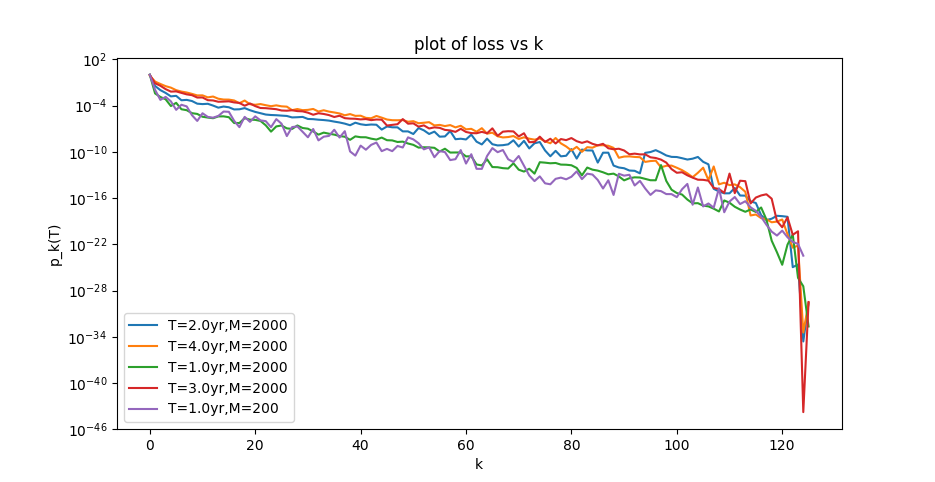
\includegraphics[width=\textwidth]{IPS_all_years}
	\caption{Plot of default probabilities for each level and maturity times
	based on IPS}
	\label{fig:IPS_all}
\end{figure}

\begin{figure}
	\centering
	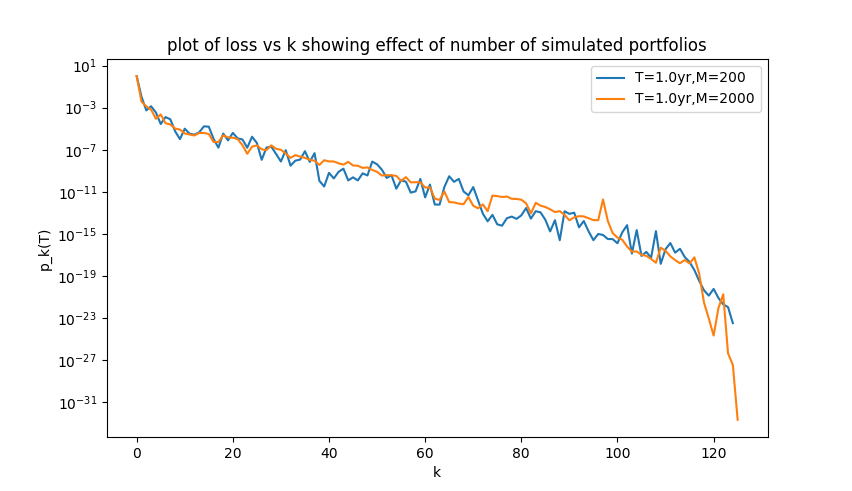
\includegraphics[width=\textwidth]{IPS_M_comparison}
	\caption{Plot comparing default probabilities for maturity $T=1$ with
	different number of portfolios}
	\label{fig:IPS_comparison}
\end{figure}

\begin{figure}
	\centering
	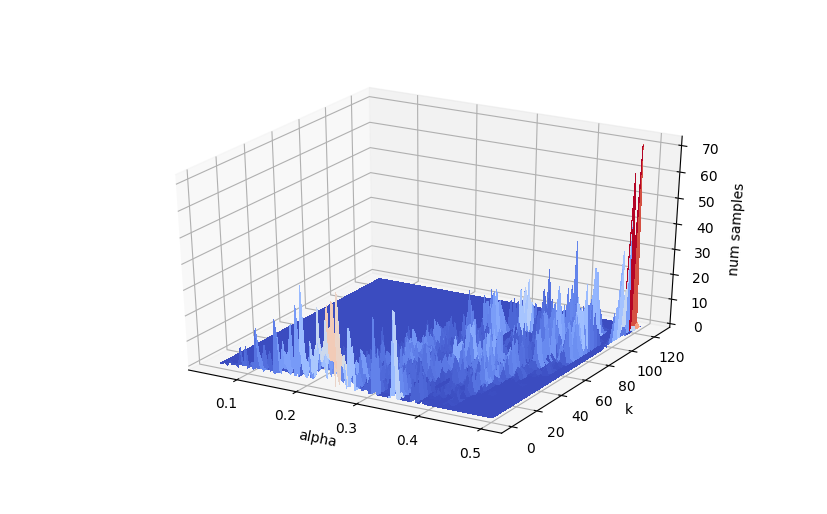
\includegraphics[width = \textwidth]{IPS_surface}
	\caption{Plot of number of defaults simulated for $\alpha$, $k$ combination}
	\label{fig:IPS_surface}
\end{figure}

\begin{figure}
	\centering
	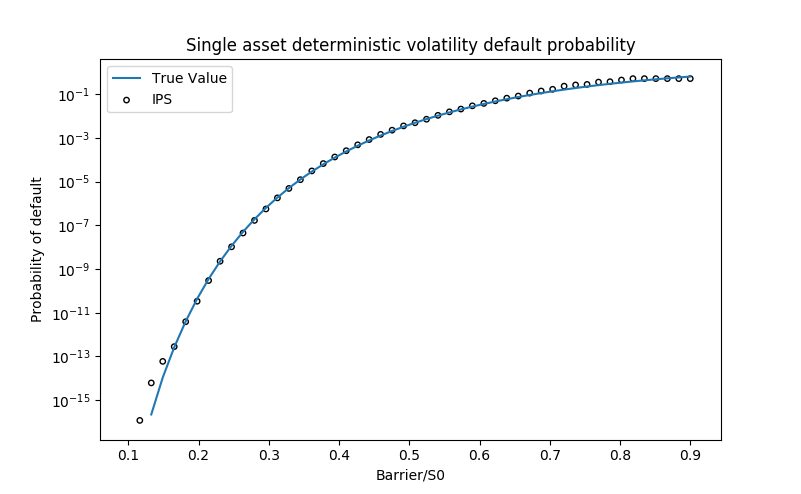
\includegraphics[width = \textwidth]{IPS_single}
	\caption{Default probabilities of different barrier levels for single asset
	deterministic volatility case}
	\label{fig:IPS_single}
\end{figure}


\clearpage
\bibliography{references}
\end{document}
